\documentclass[11pt]{article}
\usepackage{amsmath,graphicx,color,epsfig,physics}
%\usepackage{pstricks}
\usepackage{float}
\usepackage{subfigure}
\usepackage{slashed}
\usepackage{color}
\usepackage{multirow}
\usepackage{feynmp}
\usepackage[top=1in, bottom=1in, left=1.2in, right=1.2in]{geometry}
\begin{document}
\title{Particle physics HW1}
\author{Yang Ma}

\maketitle


\section{ }
Have ordered.

\section{ }

I checked PDG and collected the data into Tab.\ref{tb:bosons}, Tab.\ref{tb:quarks}, Tab.\ref{tb:lep}, Tab.\ref{tb:bm}.
\begin{table}[htb]
  \centering
  \caption{Gauge bosons and Higgs boson in Standard Model.}
  \label{tb:bosons}
  \begin{tabular}{|c|c|c|c|c|c|}
  \hline
                 & photon ($\gamma$) & gluon (g) & $W^{\pm}$             & Z                       & Higgs (H)            \\ \hline
  m (GeV)        &$<1\times 10^{-27}$ & 0         & $80.385 \pm 0.015$ & $91.1876 \pm 0.0021$ & $125.09 \pm 0.24$ \\ \hline
  $\Gamma$ (GeV) & stable            & -         & $2.085 \pm 0.042$  & $2.4952 \pm 0.0023$  & $< 0.013$         \\ \hline
  $Q$            & $< 1\times 10^{-35} e$       & 0         & $\pm e$               & 0                       & 0                    \\ \hline
  Spin           & 1                 & 1         & 1                     & 1                       & 0                    \\ \hline
  \end{tabular}
\end{table}

\begin{table}[htb]
  \centering
  \caption{Quarks in Standard Model.}
  \label{tb:quarks}
  \begin{tabular}{|c|c|c|c|c|c|c|}
  \hline
                  & u                                 & d                                 & c               & s                                 & t                      & b                      \\ \hline
  m (GeV)        & $2.2^{+0.6}_{-0.4}\times 10^{-3}$ & $4.7^{+0.5}_{-0.4}\times 10^{-3}$ & $1.28 \pm 0.03$ & $9.6^{+0.8}_{-0.4}\times 10^{-2}$ & $173.1 \pm 0.6 $       & $4.18^{+0.04}_{-0.03}$ \\ \hline
  $\Gamma$ (GeV) & -                                 & -                                 & -               & -                                 & $1.41^{+0.19}_{-0.15}$ & -                      \\ \hline
  $Q$            & $\frac{2}{3}e$                    & $-\frac{1}{3}e$                   & $\frac{2}{3}e$  & $-\frac{1}{3}e$                   & $\frac{2}{3}e$         & $-\frac{1}{3}e$        \\ \hline
  Spin           & $\frac{1}{2}$                     & $\frac{1}{2}$                     & $\frac{1}{2}$   & $\frac{1}{2}$                     & $\frac{1}{2}$          & $\frac{1}{2}$          \\ \hline
  \end{tabular}
\end{table}


\begin{table}[htb]
  \centering
  \caption{Leptons in Standard Model.}
  \label{tb:lep}
  \begin{tabular}{|c|c|c|c|c|c|c|}
  \hline
          & e                               & $\mu$                                     & $\tau$                          & $\nu_e$            & $\nu_\mu$         & $\nu_\tau$         \\ \hline
  m (MeV) & $0.5109989461$ & $105.6583745$               & $1776.86 \pm 0.12$              & $<2\times 10^{-6}$ & $<2\times10^{-6}$ & $<2\times 10^{-6}$ \\ \hline
  $\tau$  & $>6.6 \times 10^{28} yr$      & $2.1969811 \times 10^{-6} s$ & $2.903 \times 10^{-13} s$ &           -         &         -          &    -                \\ \hline
  $Q$     & -$e$                              & -$e$                                        & -$e$                              & 0                  & 0                 & 0                  \\ \hline
  Spin    & $\frac{1}{2}$                   & $\frac{1}{2}$                             & $\frac{1}{2}$                   & $\frac{1}{2}$      & $\frac{1}{2}$     & $\frac{1}{2}$      \\ \hline
  \end{tabular}
\end{table}


\begin{table}[htb]
  \centering
  \caption{Several baryons and mesons in Standard Model. }
  \label{tb:bm}
  \begin{tabular}{|c|c|c|c|c|}
  \hline
            & p             & n              & $\pi^+$                  & $\pi^0$                \\ \hline
  m (MeV)   & 938.272081    & 939.565413     & 139.57061                & 134.9770               \\ \hline
  $\tau$ &$2.1 \times 10^{29} yr$        & $880.2 \pm1.0 s$ & $2.6033 \times 10 ^{-8} s$ & $8.52 \times 10^{-17} s$ \\ \hline
  $Q$       & $+e$          & 0              & $+e$                     & 0                      \\ \hline
  Spin      & $\frac{1}{2}$ & $\frac{1}{2}$  & 0                        & 0                      \\ \hline
  \end{tabular}
\end{table}
  
\section { }
\begin{itemize}
  \item If the time evolution of state $\ket{\psi(t)}$ is
  \begin{eqnarray}
    \ket{\psi(t)}=e^{-iEt}\ket{\psi(0)},
  \end{eqnarray} 
  then we can verify that
  \begin{eqnarray}
    i \frac{d}{dt} \ket{\psi(t)}=i(-i E) e^{-iEt}\ket{\psi(0)}  = E e^{-iEt}\ket{\psi(0)} = E \ket{\psi(t)}.
  \end{eqnarray}
  Above equation is the Schrodinger equation.
  \item With the definitions in the homework question, we can directly write out 
  \begin{eqnarray}
    \tau&=&\frac{\int_0^\infty t e^{-t\Gamma} dt}{\int_0^\infty  e^{-t\Gamma} dt}= \frac{\frac{1}{\Gamma^2}\int_0^\infty \Gamma t e^{-t\Gamma} d\Gamma t} {\frac{1}{\Gamma}\int_0^\infty \Gamma t e^{-t\Gamma} d\Gamma t} \nonumber \\
    &=&\frac{-\frac{1}{\Gamma}\left [(\Gamma t e^{-\Gamma t})|_0^\infty-e^{-\Gamma t}|_0^\infty  \right]}{e^{-\Gamma t}|_0^\infty}=\frac{1}{\Gamma}.
  \end{eqnarray}
\end{itemize}


\section { }
In PDG I found
\begin{eqnarray}
  \hbar= 6.582 \times 10^{-22} {\rm MeV~s},
\end{eqnarray} 
so we can then have
\begin{eqnarray}
  1 {\rm GeV}^{-1}= 6.582 \times 10^{-22} {\rm s},
\end{eqnarray}
by setting $\hbar=1$.
Using above relations, we can obtain the lifetimes in Tab.\ref{tb:tau} from Tab.\ref{tb:bosons} and Tab.\ref{tb:quarks}. Also we can use $\tau=\hbar/\Gamma$ to obtain the decay widths from Tab.\ref{tb:lep} and Tab.\ref{tb:bm}. Numerical results are presented in Tab.\ref{tb:Gamma} and Tab.\ref{tb:Gamma2}. With $c=3 \times 10^{-10} cm/s = 1$ in natural unit, we then have the mean dacay length of $\mu$, $\tau$, $n$, $\pi^+$ and $\pi^0$ in Tab.\ref{tb:cm}. 

\begin{table}[]
  \centering
  \caption{Lifetimes of $W^{\pm}$, Z, H, t.}
  \label{tb:tau}
  \begin{tabular}{|c|c|c|c|c|}
  \hline
            & $W^{\pm}$              & Z                     & H                       & t                     \\ \hline
  $\tau$(s) & $3.16 \times 10^{-25}$ & $2.64\times 10^{-25}$ & $>5.06 \times 10^{-23}$ & $4.67 \times10^{-25}$ \\ \hline
  \end{tabular}
\end{table}


\begin{table}[]
  \centering
  \caption{Decay widths of $e^-$, $\mu$ and $\tau$. $p$, $n$, $\pi^+$ and $\pi^0$.}
  \label{tb:Gamma}
  \begin{tabular}{|c|c|c|c|}
  \hline
                & e                      & $\mu$                  & $\tau$                 \\ \hline
  m(GeV)        & $5 \times 10^{-4}$     & 0.105                  & 1.777                  \\ \hline
  $\Gamma$(GeV) & $3.17 \times 10^{-61}$ & $2.99 \times 10^{-16}$ & $2.27 \times 10^{-9}$ \\ \hline
  \end{tabular}
\end{table}

\begin{table}[]
  \centering
  \caption{Decay widths of $p$, $n$, $\pi^+$ and $\pi^0$.}
  \label{tb:Gamma2}
  \begin{tabular}{|c|c|c|c|c|}
  \hline
                & p                      & n                     & $\pi^+$                & $\pi^0$               \\ \hline
  m(GeV)        & 0.938                  & 0.940                 & 0.140                  & 0.135                 \\ \hline
  $\Gamma$(GeV) & $9.94 \times 10^{-62}$ & $7.48\times 10^{-28}$ & $2.53 \times 10^{-17}$ & $7.74 \times 10^{-9}$ \\ \hline
  \end{tabular}
\end{table}


\begin{table}[]
  \centering
  \caption{Mean decay length of $\mu$, $\tau$, $n$, $\pi^+$ and $\pi^0$. }
  \label{tb:cm}
  \begin{tabular}{|c|c|c|c|c|c|}
  \hline
          & $\mu$             & $\tau$               & $n$                   & $\pi^+$ & $\pi^0$               \\ \hline
  $l$(cm) & $6.6 \times 10^4$ & $8.7 \times 10^{-3}$ & $2.64 \times 10^{13}$ & 780     & $2.56 \times 10^{-6}$ \\ \hline
  \end{tabular}
  \end{table}

\section{ }
Insert $E_k=M-i\Gamma/2$ to 
\begin{eqnarray}
  |\ket{\psi}|^2=\frac{{\rm const.}}{|E_k-E|^2},
\end{eqnarray}
one will have
\begin{eqnarray}
  |\ket{\psi}|^2&=&\frac{{\rm const.}}{|M- i\Gamma/2-E|^2}\nonumber \\
  &=&\frac{{\rm const.}}{(M- E)^2+\Gamma^2/4}.
\end{eqnarray}
In the region $M-4 \Gamma <E < M+ 4\Gamma$, the E dependence of $|\ket{\psi}|$ is shown in Fig.\ref{fig.1_5}. Also, we notice that
\begin{eqnarray}
  \frac{d |\ket{\psi}|^2 }{d E}=0,~~{\rm when}~E=m,
\end{eqnarray}
which correspond with the maximum $|\ket{\psi}|^2=4/\Gamma^2$. Then we can verify $|\ket{\psi}|^2=2/\Gamma^2$ at $E=M+\Gamma/2$ and $E=M-\Gamma/2$, i.e. $\Gamma$ is the width of the half maximum of the resonance peak.

\begin{figure}[htb]
  \centering
  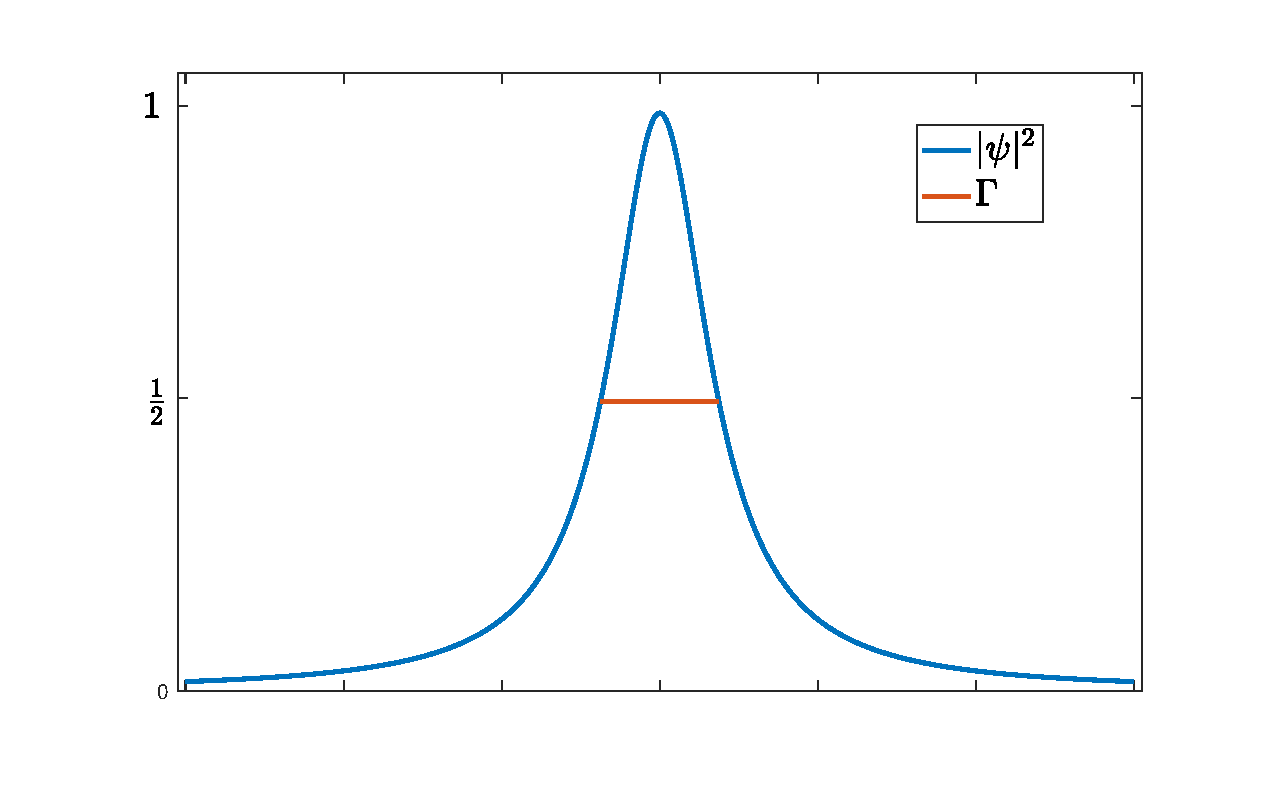
\includegraphics[width=8cm]{hw15.eps}
  \caption{E dependence of $|\ket{\psi}|$ in $M-4 \Gamma <E < M+ 4\Gamma$ .\label{fig.1_5}}
\end{figure}

\section{ }
\begin{itemize}
  \item By doing the replacement $m \to m-i\Gamma /2$ in
  \begin{eqnarray}
    \frac{1}{p^2-m^2},
  \end{eqnarray}
  we have
  \begin{eqnarray}
    \frac{1}{p^2-(m-i\Gamma /2)^2}&=&\frac{1}{p^2-m^2+im\Gamma + {\cal O}(\Gamma^2)}\\
    &=&\frac{1}{p^2-m^2+i \epsilon},
  \end{eqnarray}
  where we assumed that $\Gamma$ is very small comparing to m and see $\epsilon=m\Gamma$.
  \item We see that
  \begin{eqnarray}
    \frac{d}{d p^2}\frac{1}{(p^2-m^2)^2+(m\Gamma)^2}=0,~~{\rm when}~p^2=m^2,
  \end{eqnarray}
  where
  \begin{eqnarray}
    \frac{1}{(p^2-m^2)^2+(m\Gamma)^2}\big |_{\rm max}=\frac{1}{(m\Gamma)^2}.
  \end{eqnarray}
  Then we can easily verify that 
  \begin{eqnarray}
    \frac{1}{(p^2-m^2)^2+(m\Gamma)^2}=\frac{1}{2(m\Gamma)^2},
  \end{eqnarray}
  when $p^2=m^2\pm m\Gamma$, i.e. $m\Gamma$ is the half width of the resonance at the half maximum when it is expressed in terms of $p^2$.
\end{itemize}




\end{document}